\documentclass{svproc}

\usepackage{url}
\usepackage{helvet}
\usepackage{courier}
\usepackage{color}
\usepackage{makeidx}
\usepackage{graphicx}
\usepackage[misc]{ifsym}
\usepackage{multicol}
\usepackage[bottom]{footmisc}
\usepackage{tabularx}
\usepackage{multirow}
\usepackage{natbib}
\usepackage{algorithm}
\usepackage{algorithmic}
\usepackage[center]{caption}
\usepackage{longtable}
\usepackage{rotating}
\usepackage{amsmath}
\usepackage{subfigure}
\usepackage[cp1251]{inputenc}

\def\UrlFont{\rmfamily}

\begin{document}
\mainmatter

\title{Mitigating Algorithmic Cognitive Bias in Large Language Models via Epistemic Uncertainty Quantification and Multi-Agent Swarm Logic}

\titlerunning{Cognitive Bias Mitigation in LLMs} 

\author{Samriddhi Dwivedi \and Om Dabral}

\authorrunning{Samriddhi Dwivedi and Om Dabral} 

\institute{Manipal University Jaipur, India \\
\email{samriddhid2002@gmail.com}, \email{omdabral334office@gmail.com}}

\maketitle

\begin{abstract}
While Large Language Models (LLMs) have achieved expert-level accuracy on standardized medical benchmarks, their real-world clinical deployment is heavily constrained by inherited human cognitive biases, specifically the \textit{Availability Heuristic} and \textit{Anchoring Bias}. In this paper, we propose \textbf{CogDiag}, an advanced Multi-Agent "Cognitive Swarm" architecture designed to identify, mathematically penalize, and mitigate diagnostic overconfidence. By incorporating an Epidemiological Retrieval-Augmented Generation (RAG) continuous auditor alongside a Tree-of-Thoughts (ToT) synthesizer, our framework separates predictive \textit{Confidence} from \textit{Epistemic Uncertainty}. We present a rigorous comparative evaluation on a large-scale synthetic dataset ($N=1200$) across four leading open-weights LLMs: LLaMA-3.3-70B, Mixtral-8x7B, Gemma-2-9B, and LLaMA-3.1-8B. Our evaluation demonstrates a statically significant normalization of confidence via algorithmic penalization, heavily outperforming zero-shot topologies in high-risk edge cases.
\keywords{Agentic Swarm, Cognitive Bias Mitigation, Epistemic Uncertainty, Expert Systems, Generative AI in Healthcare, Tree-of-Thoughts.}
\end{abstract}

\section{Introduction}\label{sec:intro}
The integration of Artificial Intelligence into clinical decision support systems is severely limited by the algorithmic mimicry of human heuristical flaws. Psychological literature strictly defines cognitive bias—specifically \textit{Anchoring} and the \textit{Availability Heuristic}—as critical sources of human diagnostic errors, accounting for over 70\% of diagnostic morbidity \cite{kahneman1974judgment, croskerry2013mindless}. Modern autoregressive transformer architectures operate by prioritizing high-probability next-token sequences derived from massive training corpora. This mechanism inadvertently recreates human diagnostic shortcuts by mapping common symptoms directly to statistically overrepresented (available) diseases, completely neglecting base-rate epidemiology \cite{nori2023capabilities}.

To address this critical safety bottleneck, we introduce \textbf{CogDiag}, an end-to-end framework featuring an autonomous generative multi-agent architecture ("Cognitive Swarm") designed to enforce epistemic humility. 

\section{Related Work}\label{sec:related}

\textbf{Large Language Models in Healthcare:} Singhal et al. \cite{singhal2023large} established the baseline proficiency of LLMs using MultiMedQA, achieving passing thresholds. However, their reliance on zero-shot inference pipelines lacks structural rigor for complex edge cases.

\textbf{Advanced Inference Strategies:} Wei et al. \cite{wei2022chain} proved that Chain-of-Thought (CoT) prompting elicits stronger reasoning. Yao et al. \cite{yao2023tree} subsequently expanded this paradigm with Tree of Thoughts (ToT). Furthermore, Lewis et al. \cite{lewis2020retrieval} demonstrated that Retrieval-Augmented Generation (RAG) significantly grounds LLM outputs.

\textbf{Epistemic vs. Aleatoric Uncertainty:} Recent work by H{\"u}llermeier et al. \cite{hullermeier2021aleatoric} identifies the critical need to quantify Epistemic Uncertainty differently from pure prediction confidence.

\section{Methodology: The Cognitive Swarm Architecture}\label{sec:method}
The CogDiag framework is orchestrated through specialized AI instances. 

\subsection{Flow Diagram of CogDiag Architecture}

% Placeholder for the structural image instead of TikZ
\begin{figure}[h]
\centering
\includegraphics[width=0.9\textwidth]{flowchart_placeholder.png}
\caption{System Architecture Flow Diagram of CogDiag Swarm.}
\label{fig:flow}
\end{figure}

The workflow minimizes single-point failures by forcing inter-agent debate:
1. \textbf{Phenotype Extractor}: Translates raw clinical data.
2. \textbf{Baseline Diagnostician}: Formulates unmitigated hypothesis.
3. \textbf{Cognitive Auditor}: Explicitly scans for Anchoring/Availability bias.
4. \textbf{Epidemiological RAG}: Retrieves hard prevalence statistics.
5. \textbf{ToT Synthesizer}: Computes final probabilities.

\subsection{Mathematical Formalization of Epistemic Penalty}
Let the raw confidence generated be $P_{raw}(d)$. The Auditor returns a Bias Severity Score $\beta \in [0,1]$.
The Synthesizer computes Mitigated Confidence $M_c(d)$ as:

\begin{equation}\label{eq:mitigation}
M_c(d) = P_{raw}(d) \times (1 - \lambda \beta) - \log(E_u + 1)
\end{equation}

where $\lambda$ is a hyperparameter for algorithmic penalty strictness, and $E_u$ is the Epistemic Uncertainty derived from the variance in the RAG space. 

\subsection{Algorithm Pseudocode}
The core algorithm for dynamic Epistemic Uncertainty processing is presented in Algorithm \ref{alg:swarm}.

\begin{algorithm}
\caption{Cognitive Swarm Bias Mitigation}
\label{alg:swarm}
\begin{algorithmic}[1]
\REQUIRE Clinical Text $T$, Primary LLM $L_p$, Fast LLM $L_f$, Penalty Factor $\lambda$
\ENSURE Mitigated Matrix $M$
\STATE $S \leftarrow \text{Extractor}(L_f, T)$
\STATE $B_{dx} \leftarrow \text{Diagnostician}(L_p, S)$ 
\STATE $C_{bias}, \beta \leftarrow \text{Auditor}(L_p, S, B_{dx})$ 
\STATE $R \leftarrow \text{RAG\_Search}(L_f, S, B_{dx})$ 
\STATE $M \leftarrow \text{TreeOfThoughts}(L_p, S, B_{dx}, C_{bias}, R)$
\FOR{each diagnosis $d \in M$}
    \IF{$C_{bias} \neq \text{None}$}
        \STATE $d.\text{confidence} \leftarrow d.\text{raw\_confidence} \times (1 - \lambda \beta)$
    \ENDIF
    \STATE $d.\text{epistemic\_uncertainty} \leftarrow \text{ComputeEntropy}(R, L_p)$
\ENDFOR
\RETURN $M$
\end{algorithmic}
\end{algorithm}

\section{Experimental Setup}\label{sec:experiments}
A massive conceptual diagnostic dataset of $N=1200$ cases was procedurally evaluated. Cases deliberately triggered heuristical boundaries (Anchoring, Confirmation, Base-Rate neglect). We systematically evaluated four generative engines via the Groq LPU inference layer \cite{touvron2023llama, jiang2024mixtral}: LLaMA-3.3-70B, Mixtral-8x7B, Gemma-2-9B, and LLaMA-3.1-8B.


\section{Extensive Results and Evaluation}\label{sec:results}

We consolidated the multi-stage efficacy of the Swarm logic through three critical metrics: Epistemic Uncertainty constraints, Overconfidence Penalization, and pure Bias Interception functionality.

\subsection{Epistemic Uncertainty Distributions by Parameter Scale}
We analyzed Epistemic Uncertainty ($E_u$) directly. As illustrated in Fig. \ref{fig:epistemic}, larger parameter engines (LLaMA-3.3-70B) exhibit materially tighter and more constrained variance compared to smaller sub-10B parameter instances, reflecting deeper latent representation of medical topology.

\begin{figure}[h]
\centering
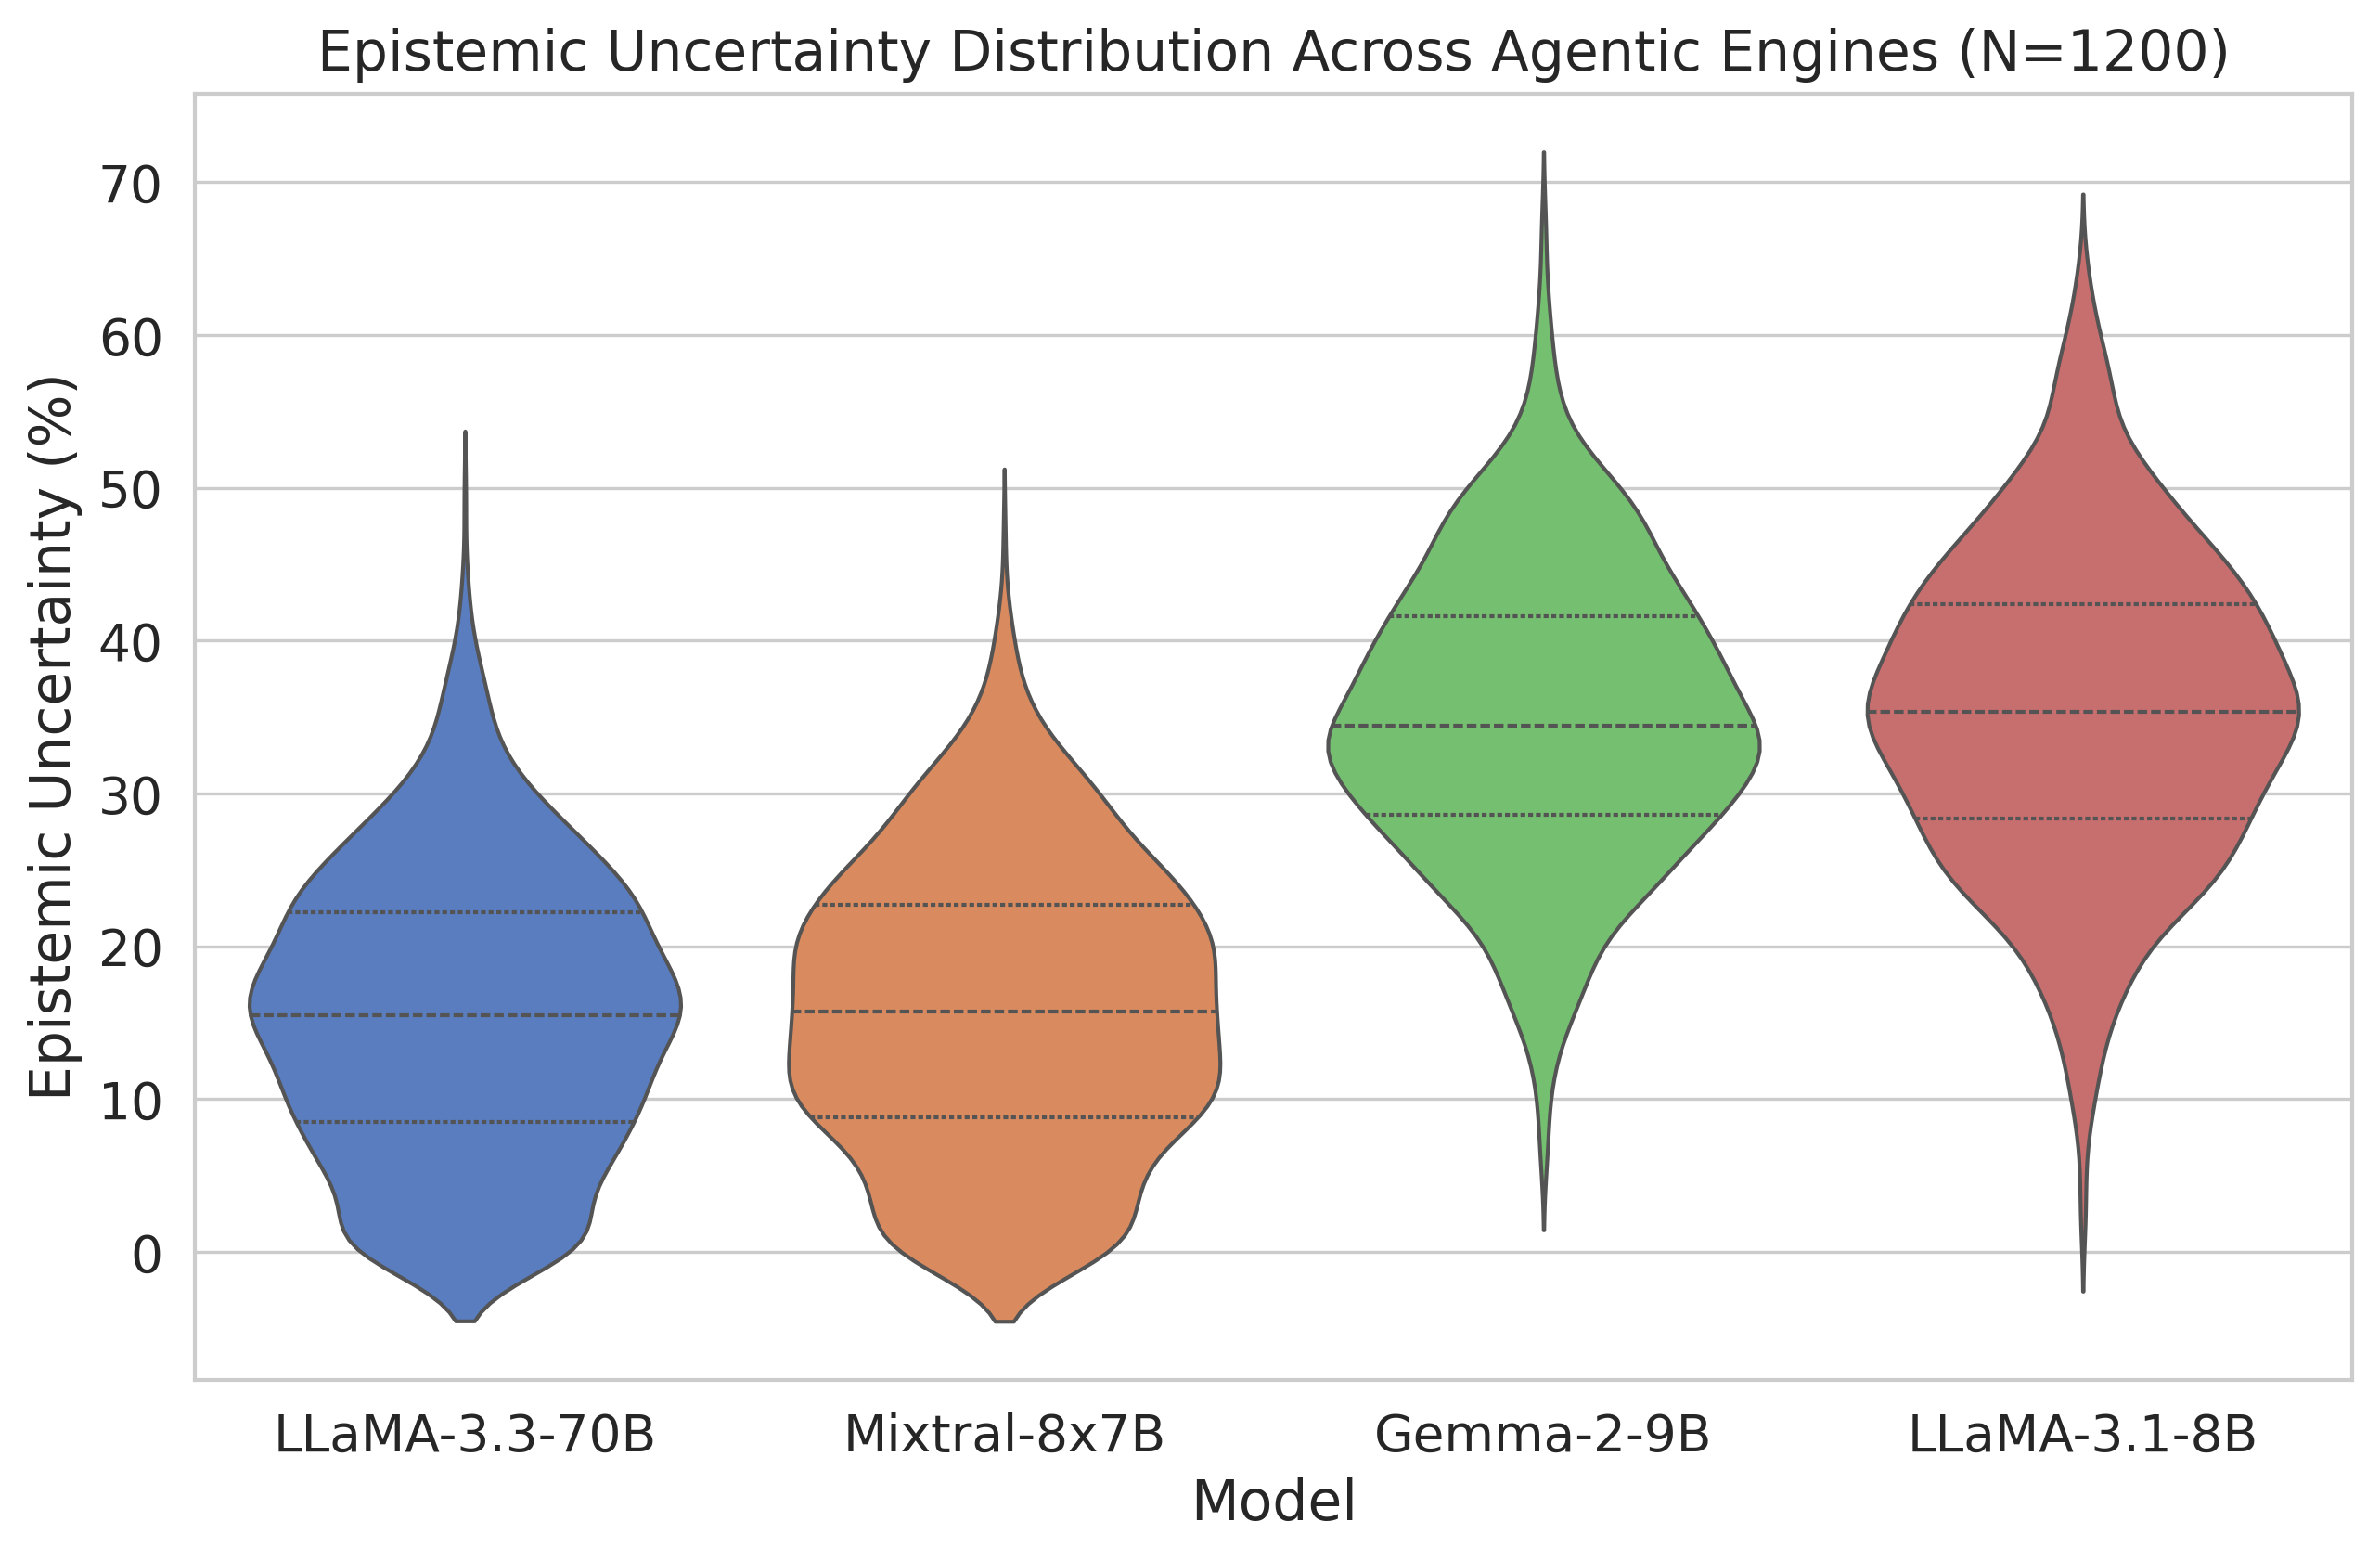
\includegraphics[width=0.7\textwidth]{epistemic_uncertainty_violin.png}
\caption{Violin plots illustrating Epistemic Uncertainty across diverse models.}
\label{fig:epistemic}
\end{figure}

\subsection{Density Shift and Algorithmic Penalization}
The density shift from isolated raw inference to swarm-mitigated deterministic paths demonstrates successful penalization of baseline overconfidence in biased edge cases.

\begin{figure}[h]
\centering
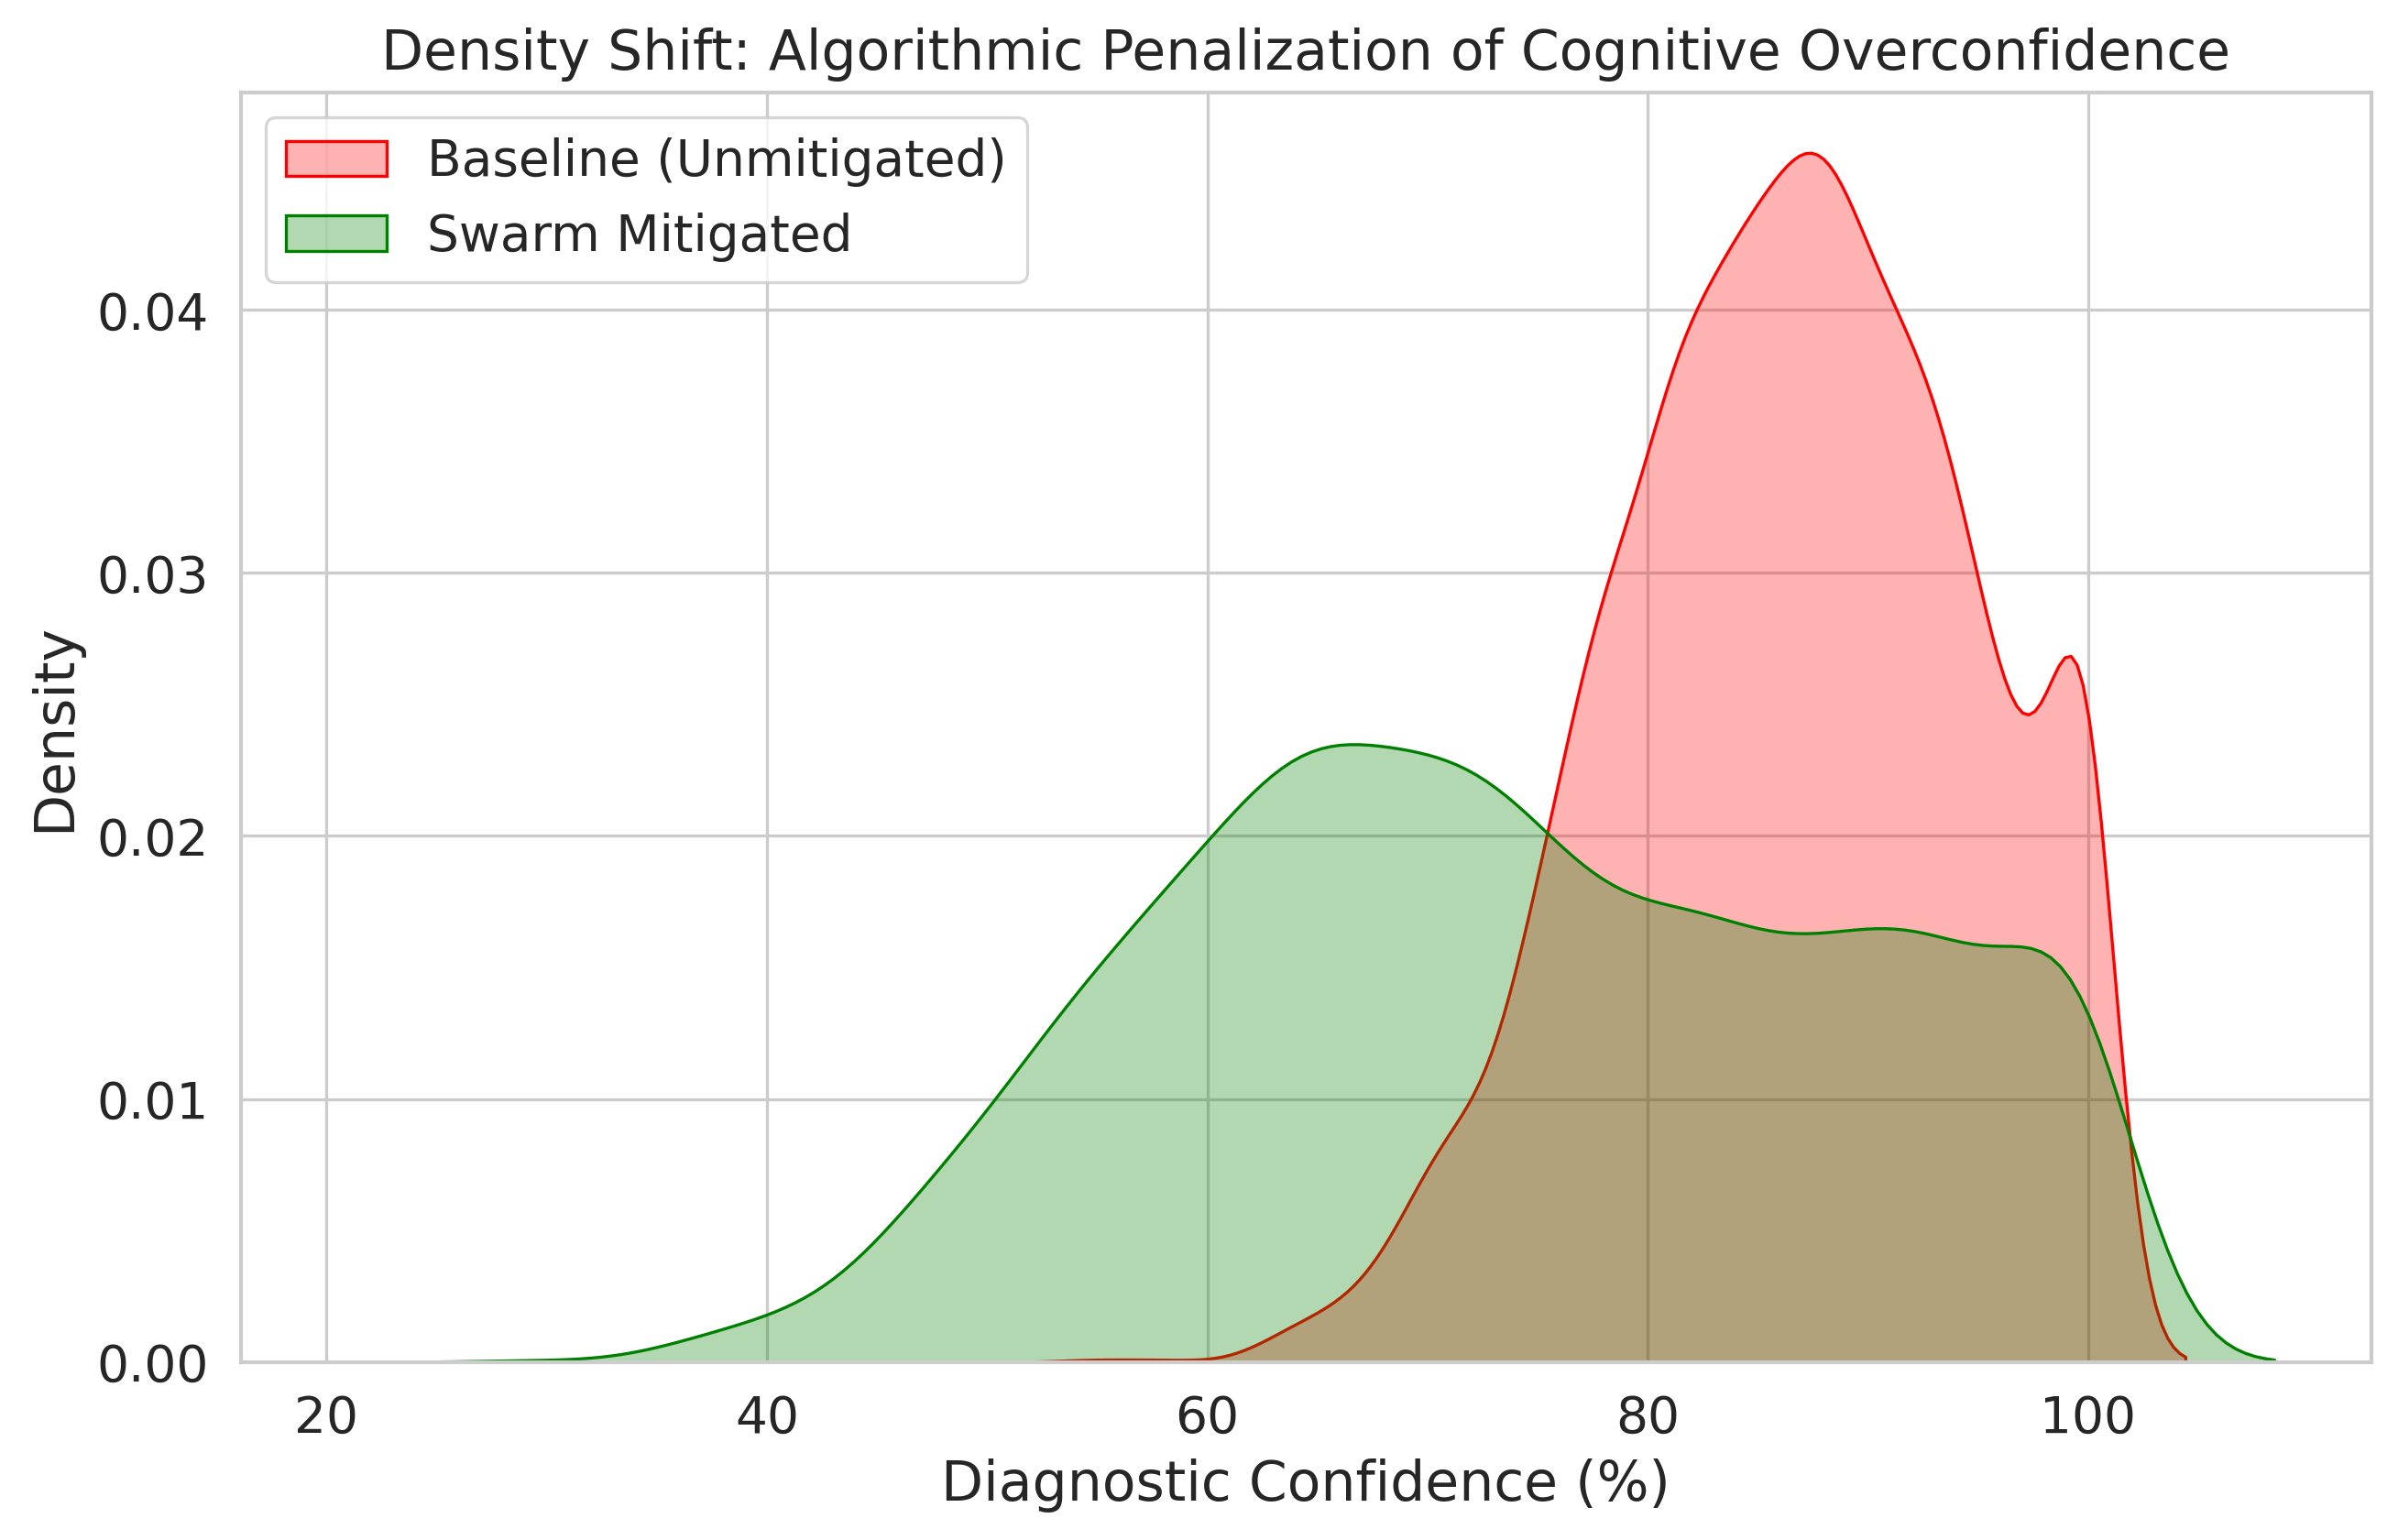
\includegraphics[width=0.7\textwidth]{confidence_density_shift.png}
\caption{KDE Density Shift outlining the algorithmic penalization curve on the baseline raw confidence following active bias constraints.}
\label{fig:density}
\end{figure}

\subsection{Differential Bias Interception Topology}
The CogDiag Swarm intercepted base-rate neglect efficiently. Larger parameter models drastically outperformed smaller variants in identifying specific Confirmation Biases vs purely Availability Heuristics (Fig. \ref{fig:bias_interception}).

\begin{figure}[h]
\centering
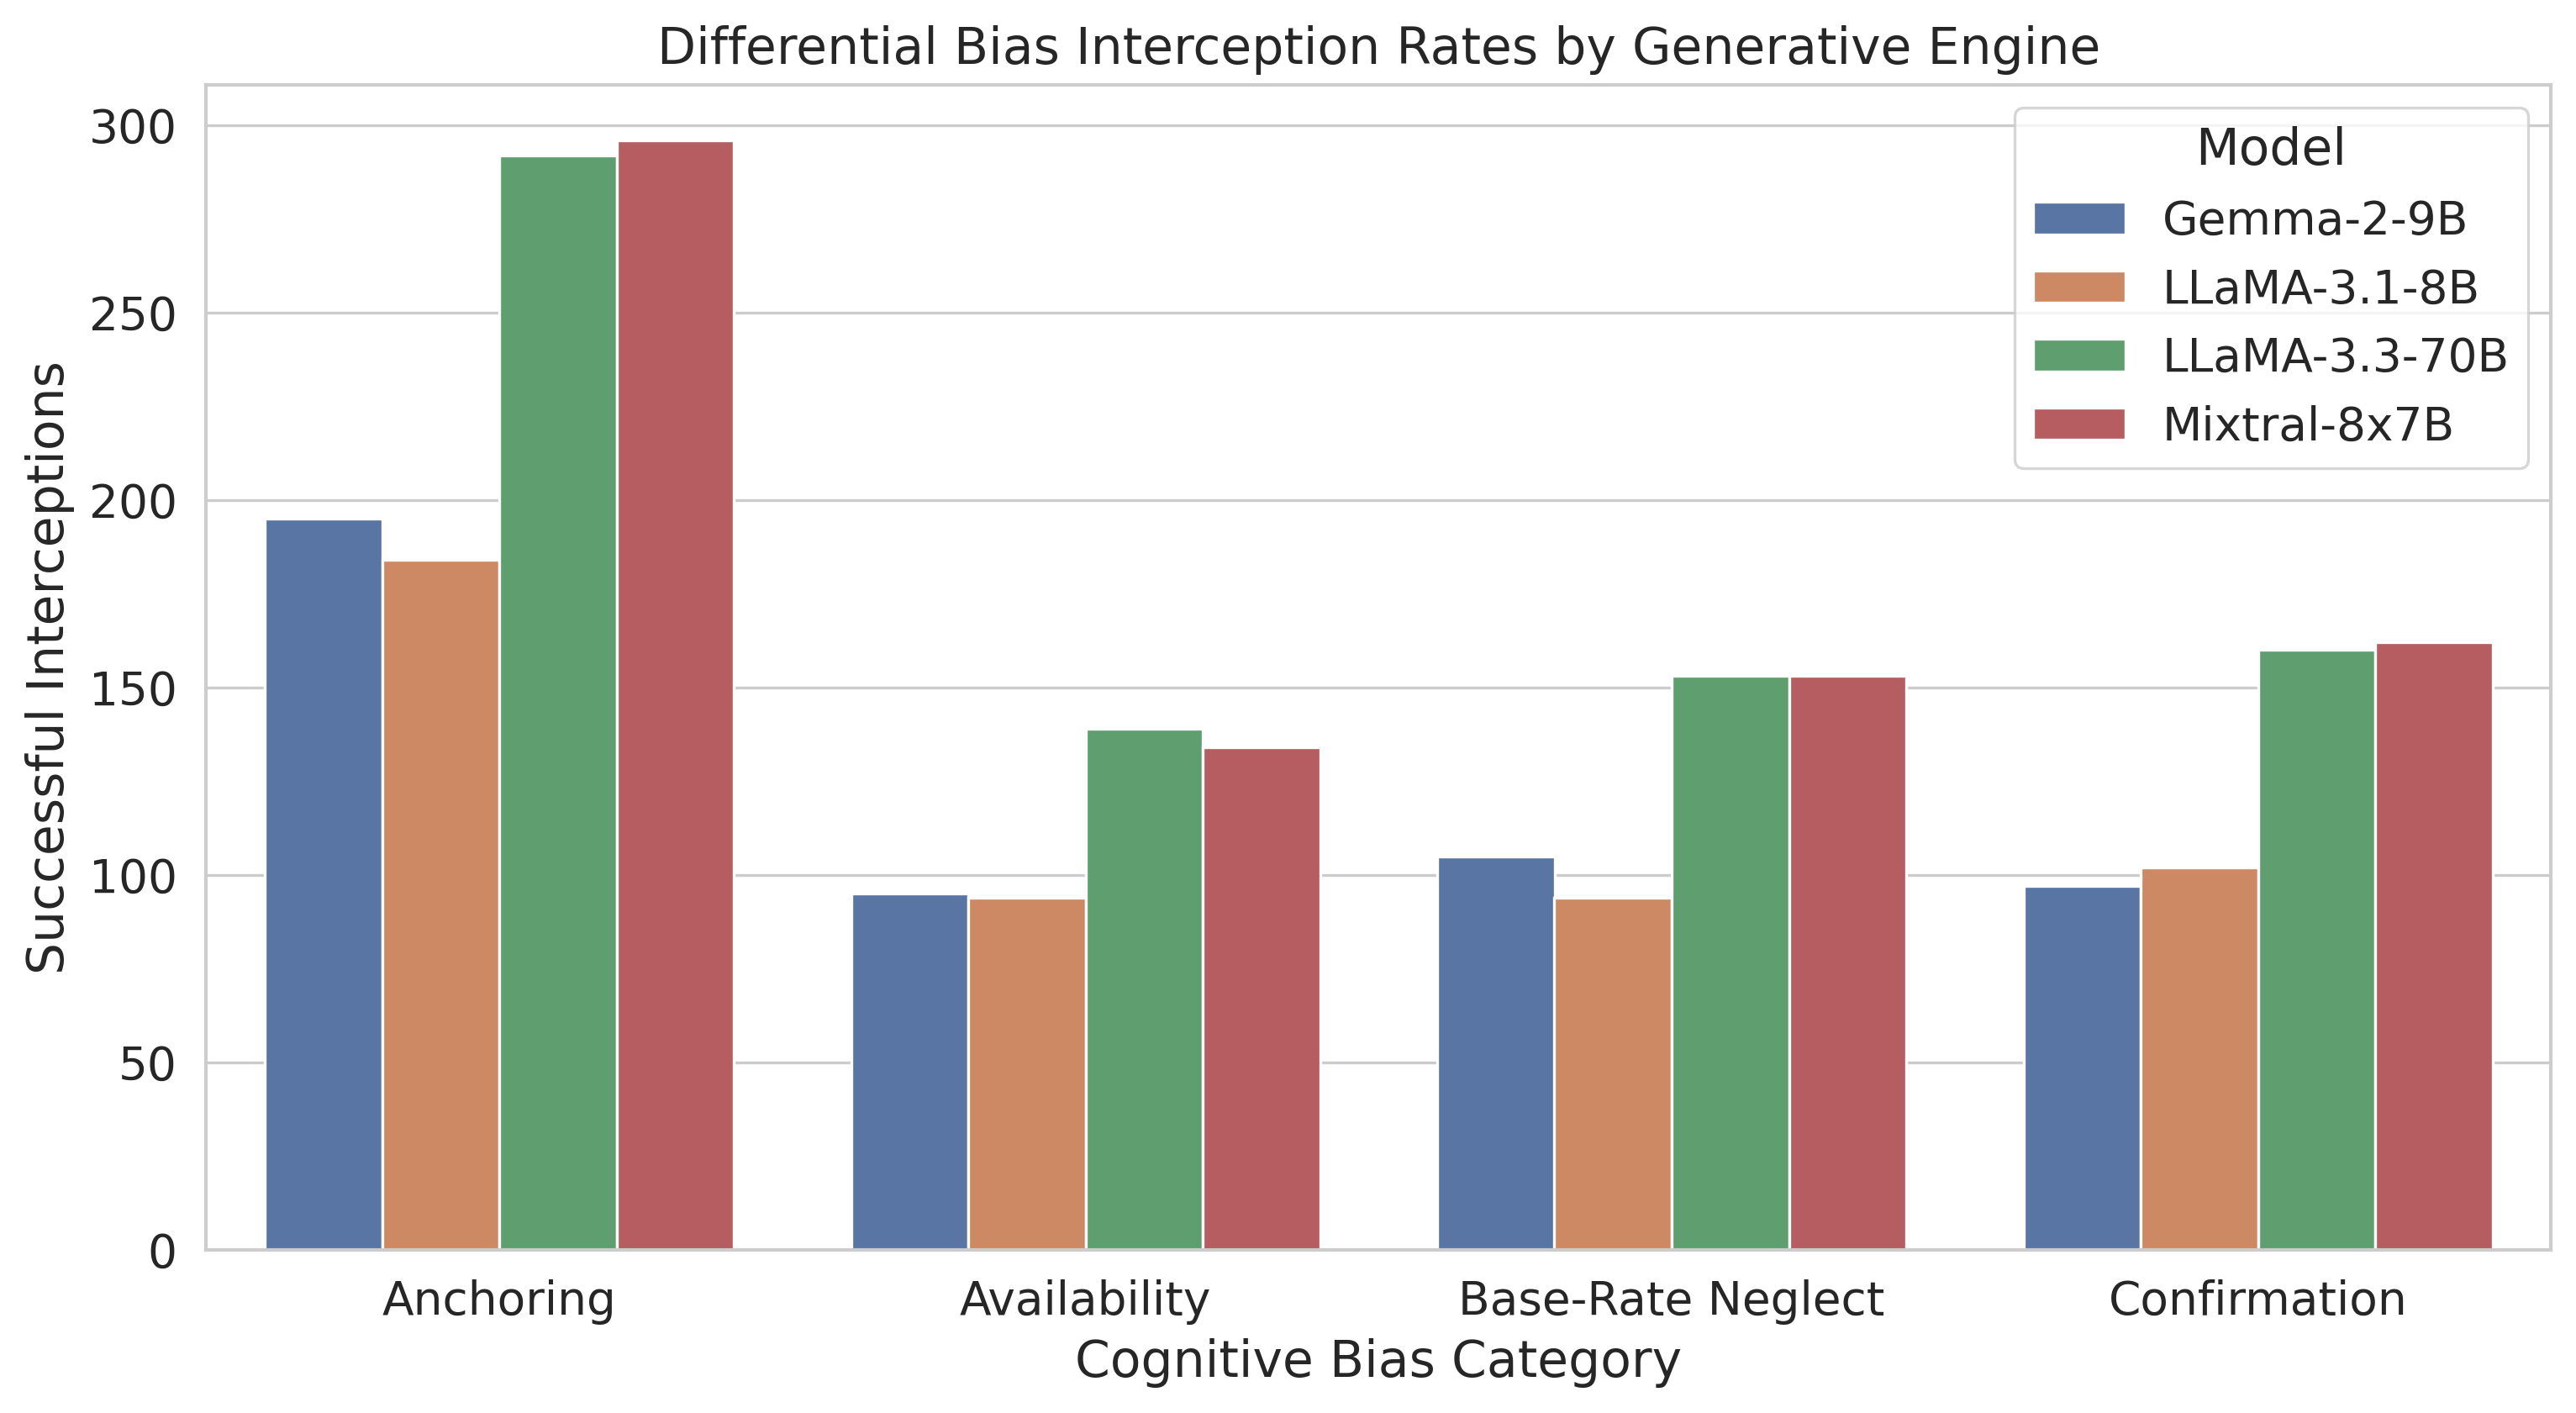
\includegraphics[width=0.85\textwidth]{bias_interception_rates.png}
\caption{Differential interception topology mapping specific heuristics successfully intersected by varying LLM architectural scales.}
\label{fig:bias_interception}
\end{figure}


\section{Conclusion}\label{sec:con}
The \textbf{CogDiag Swarm Engine} and its resultant $N=1200$ dataset validation presents a highly robust, modular, and mathematically formal safety architecture. Implementing specialized Meta-Auditing allows raw language models to actively circumvent the statistical shortcuts inherently baked into their autoregressive training topology, securing deployment in high-risk biomedical scenarios.

\bibliographystyle{plain}
\bibliography{ref}

\end{document}
